\documentclass[../main.tex]{subfiles}
\begin{document}
\chapter{Security assurance: lo stato dell'arte e la sfida}
\section{Introduzione}
In questo capitolo si approfondirà lo stato dell'arte in materia di \textbf{security assurance} e \textbf{controllo della compliance}, ovvero la verifica della conformità di un'infrastruttura informatica tradizionale, ibrida o cloud, rispetto a una politica, che può essere sviluppata internamente oppure derivata da un più complesso apparato normativo o da uno standard.
In particolare verranno trattate le problematiche di sicurezza introdotte dall'adozione di un approccio \textit{cloud}, all'interno dei processi \textit{IT} di un'organizzazione strutturata sulla base di un'infrastruttura informatica tradizionale.

Spesso si fa coincidere il concetto di \texit{cloud computing} con quello di \texit{outsourcing}, di fatto presupponendo che l'adozione di tecnologie \textit{cloud} corrisponda all'attitudine di concedere a terzi gli oneri di gestione di una parte dell'infrastruttura informatica.
La definizione di \textit{cloud computing} a cui si fa riferimento in questo elaborato di tesi è quella del NIST\footnote{National Institute of Standards and Technology, \textit{http://www.nist.org/}} nel documento \textit{SP-800-145}\cite{NISTCloud} nel quale il cloud è presentato come un insieme di tecnologie aventi come obiettivo l'erogazione di servizi e risorse in modalità \textit{on-demand} da un pool condiviso.
La condizione di \textit{outsourcing}, quindi, acquisisce una connotazione non strettamente necessaria all'adozione del servizio \textit{cloud}, con cui tuttavia condivide alcuni vantaggi\cite{OutsourcingCloud} soprattutto per realtà dove il \textit{core business} non è il settore IT:
\begin{enumerate}
\item Contenimento dei costi
\item Velocità nel ciclo di sviluppo
\item Garanzia di prestazioni e di qualità
\item Servizio distribuito geograficamente
\item Contratti di affitto strutturati e dimensionati
\end{enumerate}

\section{Sicurezza nel cloud computing}
Lo scopo finale dell'utilizzo di tecnologie \textit{cloud} consiste nella possibilità per un'organizzazione di usufruire di un modello scalabile, elastico, standard, misurabile e orchestrabile al fine di poter garantire continuità di servizio e prestazioni elevate, demandando la gestione dei processi sistemistici a piattaforme centralizzate e intelligenti.
A tal proposito il NIST\cite{NISTCloud} identifica tre modelli di servizio:
\begin{itemize}
    \item \textbf{IaaS}, \textit{Infrastructure as-a-Service}, nel quale è l'asset erogato è l'infrastruttura informatica, in termini di potenza di calcolo mediante sistemi di virtualizzazione, risorse di rete e storage. Essendo il modello più di difficile gestione, è spesso amministrato tramite un orchestratore. Esempi di tecnologie open-source in questo settore sono \textit{OpenStack}\footnote{Software open-source per la realizzazione di infrastrutture cloud pubbliche e private, https://www.openstack.org/}, \textit{oVirt\footnote{Software open-source alla base della piattaforma }}, \textit{Apache CloudStack}
    \item \textbf{PaaS}, \textit{Platform as-a-Service}, tramite il quale si fornisce all'utente la possibilità di eseguire servizi personalizzati offrendo meccanismi di contenimento nell'esecuzione, scalabilità e multi-tenancy. L'utente ha un controllo parziale sull'esecuzione del servizio: solitamente egli può interagire in modo limitato con il kernel. Una delle tecnologie più utilizzate è quella dei \textit{container}, un evoluzione del concetto di \textit{jail} proprio dei sistemi operativi BSD, il cui obiettivo è quello di utilizzare meccanismi di segregazione delle risorse basati sulle funzionalità del kernel. I servizi vengono eseguiti in un ambiente isolato, ed hanno un filesystem e uno stack di rete simulato in software dedicati. Una delle implementazioni più note della tecnologia \textit{container} è \textit{Docker}\footnote{Docker, \textit{https://www.docker.com}} che, nato inizialmente come evoluzione di LXC, è ora basato su una libreria proprietaria e costituisce la base per molte piattaforme PaaS (es. Kubernetes\footnote{Kubernetes, soluzione \textit{PaaS} progettata da Google \textit{https://kubernetes.io/}} e OpenShift\footnote{OpenShift, soluzione \textit{PaaS} di Red Hat \textit{https://www.openshift.com/}}). 
    \item \textbf{SaaS}, \textit{Software-as-a-Service}, che permette all'utente di usufruire delle funzionalità di un singolo applicativo, riducendo al minimo l'effort computazionale sulla macchina dell'utente stesso. Tipicamente in questa categoria ricadono le applicazioni web, alcune applicazioni mobile e alcuni software per PC. Alcuni esempi di \textit{SaaS} noti sono \textit{Office 365 Online}\footnote{Office 365 è la versione cloud-based della nota suite per l'ufficio \textit{Microsoft Office}, \textit{https://www.office365.com}} e \textit{Google Docs}\footnote{Google Docs è una suite per l'ufficio sviluppata da Google ed erogata esclusivamente come applicazione web, \textit{https://docs.google.com}}.
\end{itemize}
\begin{figure}[H]
\centering
\makebox[\textwidth]{
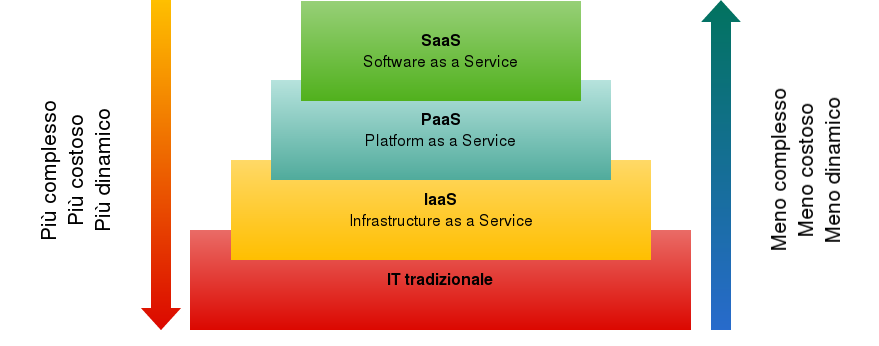
\includegraphics[width=\textwidth]{immagini/IAASPAASSAAS.png}
}:q!
\caption{Modelli di servizio}\label{fig:modelliservizio}
\end{figure}




La parola chiave è quindi \textbf{"automazione"}. Questa, oltre a garantire una solidità del modello di distribuzione di un servizio grazie a schemi dichiarativi, apporta notevoli vantaggi anche dal punto di vista della sicurezza, facilitando la gestione degli aspetti di confidenzialità, integrità e disponibilità.
\\Il paradigma \textit{as-a-service} ha infatti consentito la costituzione di una \textit{baseline} robusta garantita dalla centralizzazione delle funzionalità di security le quali, essendo erogate come risorse \textit{cloud}, sono interamente gestite dal \textit{cloud service provider} - pubblico o privato - che può demandarne la gestione parziale all'utente mediante meccanismi di orchestrazione, interfacce grafiche ed API.
\\Se a primo impatto può apparire come un enorme vantaggio, di fatto ciò introduce un \textit{single point of failure}, determinando livelli di rischio aggiuntivi rispetto alle infrastrutture tradizionali. Si pensi, ad esempio, alle funzionalità di \textit{firewalling} offerte generalmente con la denominazione di \textit{security groups} o \texit{Firewall as-a-Service} (FWaaS): un'implementazione non idonea dal punto di vista funzionale nel substrato infrastrutturale del fornitore di servizi, potrebbe determinare la mancanza di sicurezza per i servizi che ne fanno affidamento.
La stessa asserzione è valida per molte altre funzionalità comunemente offerte dal provider: cifratura dei volumi di storage, crittografia e controllo degli accessi nei servizi di block-storage e così via.


Ulteriori riflessioni possono essere fatte anche per quanto riguarda l'aspetto di integrità del dato: se da una parte il cloud service provider implementa già meccanismi di basso livello per la persistenza dello storage, ridondanza, sistemi di backup automatici, dall'altra non si ha la chiara evidenza di come questi aspetti siano effettivamente gestiti e di come la proprietà sia garantita.


Per quanto concerne la proprietà di disponibilità, la dicotomia va ricercata trattando i concetti di disponibilità del dato e disponibilità del servizio separatamente.
Il \textit{cloud computing} offre intrinsecamente solidità in quanto basato sui concetti di scalabilità, elasticità e ridondanza. Grazie ai meccanismi di orchestrazione tramite API è infatti possibile configurare le applicazioni per l'\textit{auto-scaling}, al fine di mantenere una qualità adeguata nell'erogazione del servizio al crescere degli utenti. Ciò, dal punto di vista della sicurezza, ha portato a notevoli benefici per quanto riguarda la mitigazione di attacchi DoS\footnote{Denial of Service}, garantendo la continuità di servizio riducendo i costi.
Tuttavia esistono dei prerequisiti per garantire la disponibilità: innanzitutto il \textit{cloud service provider} deve assicurare la ridondanza dei dati e della rete, contemplando l'ipotesi di distribuire le risorse su più località geografiche, con l'obiettivo sia di prevenire guasti localizzati che di erogare la risorsa dalla località più vicina rispetto all'utente.

Nel momento in cui funzionalità comunemente demandate ad hardware specifico vengono implementano in software, si determinano sia benefici che svantaggi che devono sia essere contemplati in fase di valutazione del rischio che trattati nei contratti di service level agreement. Una compromissione dell'interfaccia di gestione della piattaforma cloud, sia che si tratti di una dashboard sia che si tratti di un'interfaccia API, può portare a un'interruzione di servizio.

Gli standard di sicurezza classici, così come l'assetto normativo e i contratti di \textit{service level agreement}, necessitano di essere adeguati per supportare l'integrazione di tecnologie cloud all'interno degli stack tradizionali, tenendo conto delle problematiche di \textit{shared responsability} presentate.

Il NIST \cite{NISTCloud} riconosce quattro diversi modelli di deployment:
\begin{itemize}
    \item \textbf{Public Cloud}: modello in cui le risorse sono fornite per un utilizzo pubblico. È tipicamente erogato in outsourcing tramite la rete internet. L'hardware è in mano a un unico provider che eroga servizi in \textit{outsourcing} e ne dispone le metriche e la tariffazione.
    \item \textbf{Private Cloud}: cloud dedicata a un'azienda o organizzazione, sfruttata per erogare servizi appartenenti al provider. L'hardware è generalmente nel datacenter dell'organizzazione.
    \item \textbf{Hybrid Cloud}: approccio ibrido dato dalla composizione di public cloud e private cloud, o di public cloud e infrastrutture tradizionali. Le infrastrutture coinvolte rimangono distinte e sono legate tra loro da un'unica tecnologia (standard o proprietaria) che facilita la migrazione e la portabilità delle risorse.
    \item \textbf{Community Cloud}: modello che fornisce una cloud per uso esclusivo di una comunità di utenti appartenenti ad organizzazioni con obiettivi funzionali comuni. Può essere di proprietà di una o più organizzazioni della community, o di terze parti.
\end{itemize}
Per ognuno di questi modelli è possibile esplicitare dei requisiti da soddisfare al fine di colmare il rapporto di sfiducia proprio di questo settore\cite{Ardagna:2015:SAC:2808687.2767005}.

\section{Valutazione del rischio: vulnerabilità, minacce e attacchi}
In letteratura sono stati proposti molti lavori sulla valutazione del rischio su infrastrutture cloud. Nei paragrafi a seguire verranno discussi alcuni di questi approcci, sulla base della metodologia utilizzata da Ardagna et Al.\cite{Ardagna:2015:SAC:2808687.2767005}.
Le vulnerabilità possono essere categorizzate in tre macro aree, in base alla superficie di attacco considerata:
\begin{enumerate}
    \item \textbf{Livello applicativo}: quando l'attacco è condotto da un qualsiasi attore nei confronti di una piattaforma SaaS
    \item \textbf{Tenant su tenant}: quando l'attacco è condotto da attori appartenenti a un tenant nei confronti di un altro tenant
    \item \textbf{Provider su tenant} e \textbf{Tenant su provider}: quando l'attacco è condotto dal provider nei confronti di un tenant (tipicamente malevolo) oppure da un tenant nei confronti del provider 
\end{enumerate}
\subsection{Livello applicativo}
Si tratta di vulnerabilità tradizionali che da anni tengono sotto scacco il panorama \textit{web services}: si va da attacchi protocollari sulla comunicazione tra servizi fino alla compromissione di applicativi software specifici. Il target dell'attacco sono le piattaforme SaaS, spesso derivate dal porting di un'applicativo tradizionale sul cloud e non nativamente pensate per essere erogate online: per questo motivo sono caratterizzate da una superficie di attacco molto vasta.

Alcuni lavori significativi citati nel survey di rifermento \cite{Ardagna:2015:SAC:2808687.2767005} sono:
\begin{itemize}
    \item \textbf{Gruschka and Iacono, 2009}\cite{Ieee5175877}, nel quale è stato presentato un \textit{replay attack}, sfruttando una vulnerabilità del meccanismo di verifica della firma digitale sull'interfaccia SOAP di \textit{Amazon EC2}, e sono state eseguiti comandi sulle API con i privilegi di un utente legittimo
    \item \textbf{Bugiel et Al., 2011}\cite{Bugiel:2011:AES:2046707.2046753}, che hanno analizzato le minacce sulla confidenzialità e la privacy estraendo con successo informazioni sensibili da immagini di macchine virtuali Amazon 
\end{itemize} 

\subsection{Tenant su tenant}
Le vulnerabilità \textit{tenant su tenant} sono tipiche dei sistemi virtualizzati, quando tenant differenti condividono la stessa infrastruttura e, più specificatamente, lo stesso hardware fisico: gli attacchi possono avvenire per configurazioni erronee o vulnerabilità sull'infrastruttura di virtualizzazione. Si tratta quindi di attacchi che avvengono al livello più basso dello stack cloud\cite{Ardagna:2015:SAC:2808687.2767005}.

Alcuni contributi interessanti per questa categoria di attacchi e vulnerabilità sono quelli di:

\begin{itemize}
    \item \textbf{Ristenpart et al}, 2009\cite{Ristenpart:2009:HYG:1653662.1653687}, in cui è discusso un attacco alla confidenzialità delle informazioni relative a istanze di servizi in esecuzione. L'attacco dimostrato è basato sul fatto che i servizi sono ospitati sullo stesso hardware, per cui per un servizio è possibile generare traffico e monitorare le proprie performance per fare inferenza su quelle di un altro servizio.
	\item \textbf{Green}\cite{Ieee6427814}, che propone un ulteriore attacco di tipo \textit{side-channel} che coinvolge, questa volta, due virtual machine ospitate sullo stesso hardware.
\end{itemize}
\subsection{Provider su tenant, tenant su provider}
Le vulnerabilità di questo tipo si verificano ogni qual volta un utente o un'organizzazione sposta le proprie risorse su un'infrastruttura cloud non fidata - nella quale il provider è malevolo oppure semplicemente curioso - oppure nel caso in cui l'utente inizia ad usare un servizio cloud con l'obiettivo di attaccare il provider (ad esempio creando botnet per lanciare attacchi denial of service, attaccando le API di orchestrazione e così via) \cite{Ardagna:2015:SAC:2808687.2767005}.


Le tipologie di attacchi che sfruttano queste vulnerabilità, sono generalmente rivolte al livello IaaS\cite{Ardagna:2015:SAC:2808687.2767005}, ma non è esclusa la possibilità di attacchi a livello PaaS e SaaS.

Il survey si sofferma sul lavoro Huan Liu\cite{Liu:2010:NFD:1866835.1866849}, il quale illustra una attacco DDoS basato sulla saturazione della banda della rete virtuale: la virtualizzazione dello stack di rete a livello software (\textit{software-defined network}) richiede, oltre a risorse di rete, anche un'elevata capacità di calcolo.


Le vulnerabilità provider su tenant sono invece trattate da Rocha e Correira\cite{Ieee5958798} che propongono una panoramica dei possibili attacchi alla confidenzialità - che possono essere condotti anche dal fornitore di servizi - discutendone le contromisure, e da Bleikertz et al. \cite{Bleikertz:2013:CCC:2524523.2524526} che si concentrano sulla problematica di proteggere i clienti da attacchi condotti da provider esterni, fornendo un'architettura \textit{Cryptography as-a-Service client-driven}.


La problematica di confidenzialità nella casistica \textit{provider-on-tenant} è anche l'oggetto di De Capitani di Vimercati et. al\cite{Ieee7134727} in cui è descritta una tecnica per preservare la confidenzialità del dato riallocandolo in modo dinamico ad ogni accesso su tre nodi, risolvendo così anche i problemi di collusione tra i service provider coinvolti.
Un ulteriore articolo di De Capitani di Vimercati et al\cite{Ieee6681865}. affronta la problematica del provider \textit{onesto ma curioso} con una soluzione per l'integrità dei risultati delle query di join, che discute la casistica di un server di storage di terze parti e di fornitori di potenza di calcolo esterni e malevoli i quali producono i risultati del join per basi di dati ospitate esternamente.


\section{Tecniche di sicurezza per la cloud}
Data l'etereogeneità delle problematiche e degli approcci adottati negli articoli citati, è possibile affermare che garantire proprietà di sicurezza in ambienti cloud è molto impegnativo: questi lavori presentano solamente soluzioni parziali al problema, affrontando di volta in volta problemi specifici e presentando tecniche sviluppate \textit{ad-hoc}\cite{Ardagna:2015:SAC:2808687.2767005}.
Saranno di seguito presentati alcuni approcci e tecniche per garantire la sicurezza su sistemi cloud.

\subsection{Autenticazione e controllo degli accessi}
I sistemi tradizionali per l'autenticazione e il controllo degli accessi si sono verificati inefficienti per la cloud, pertanto è stato necessario definire nuovi approcci. L'adozione di nuovi \textit{pattern} di sviluppo orientati alla scalabilità - come ad esempio il pattern \textit{micro-services}, naturale evoluzione delle architetture SOA - ha reso necessario sviluppare meccanismi di autenticazione decentralizzati e federati.
Almulia and Yeun [2010] offrono una panoramica sui protocolli di autenticazione e \textit{identity management}, analizzandone la sicurezza, l'effort implementativo e i costi\cite{Ieee5542654}.

Costituendo parte critica per la maggior parte dei sistemi, i servizi di autenticazione, gestione dell'identità e gestione delle policy di accesso sono erogati \textit{as-a-service}.

Takabi e Joshi hanno descritto un sistema di gestione delle policy \textit{as-a-service} (PMaaS, \textit{Policy Management as-a-service}) che fornisce un punto di controllo centralizzato indipendente dalla locazione della risorsa\cite{pittir13526}.
Prima di accedere a una risorsa è necessario contattare il server di autenticazione e autorizzazione centralizzato che rilascerà il \textit{grant} dopo opportuna verifica.
\textit{Azure Active Directory}, il porting \textit{SaaS} di \texit{Microsoft Active Directory}, provvede sia a funzionalità di autenticazione che di policy management e fornisce alcuni driver di integrazione per la maggior parte dei protocolli noti.


Tuttavia, poiché molte realtà complesse dispongono già di meccanismi di autenticazione mediante \textit{ticket granting} isolate dalla rete Internet, sono stati ideati anche modalità di autenticazione e controllo degli accessi completamente \textit{stateless} (ad esempio OAuth).
È il caso dei \textit{JSON Web Token}, formalizzati nella RFC 7519: l'\textit{authentication server}, dopo aver validato la richiesta di autenticazione, restituisce un token \texit{JSON} firmato che contiene l'identità dell'utente e tutti i \textit{grant} per le autorizzazioni ad esso relative.
Non esiste il concetto di sessione, la validità del token è data esclusivamente da una marca temporale e da una durata. Il token può essere utilizzato quindi per autenticare le richieste verso i vari servizi, cui spetta l'onere di verificarne la validità del contenuto e della firma, decifrabile tramite segreto condiviso con il server di autenticazione che lo ha emesso.
I vantaggi di un approccio simile sono molteplici, tuttavia è impossibile revocare il token una volta emesso. Eventuali blocchi sono effettuabili tramite sistemi di \textit{blacklisting} che riporterebbero in auge la problematica della decentralizzazione che si voleva risolvere. La prassi è quindi quella di emettere token \texit{one-time} o con durata breve, al fine di minimizzare la durata di una possibile finestra temporale di attacco.

\subsection{Crittografia, firma digitale e trusted computing}
La crittografia è essenzialmente utilizzata per proteggere la confidenzialità dei dati, delle comunicazioni e le attività sensibili da tutti quegli avversari che mirano a disturbare l'operatività della cloud.
La maggior parte della letteratura utilizza tecniche di crittografia per preservare la confidenzialità: l'obiettivo di queste metodologie è di facilitare la migrazione dei dati gestiti da sistemi tradizionali verso la cloud.
Tuttavia non sono assenti tecniche focalizzate su altre proprietà di sicurezza, come l'utilizzo della firma digitale per curare gli aspetti di integrità e privacy.

\subsubsection{Trusted Computing}
Il \textit{trusting computing} è una tecnica utilizzata per effettuare computazioni sicure, basata sull'utilizzo della crittografia asimmetrica e di un dispositivo hardware dedicato (TPM, Trusted Platform Module) tramite il quale è possibile \textit{i)} identificare univocamente i dispositivi con un numero di serie e una chiave di cifratura implementata in hardware \textit{ii)} cifrare informazioni con la chiave di cifratura \textit{iii)} firmare informazioni con la chiave di cifratura.
Queste funzionalità pongono le basi per una serie di utilizzi avanzati volti a preservare l'integrità e la confidenzialità di dati - sia in transito su una rete, che memorizzati su disco o sui firmware del dispositivo - codice e hardware, riducendo o annichilendo gli effetti di eventuali attacchi.

Boampong e Wahsheh nel 2012 hanno proposto un modello per utilizzare il TPM al fine di garantire la correttezza dei processi di autenticazione, l'integrità e la confidenzialità sulla cloud\cite{Boampong:2012:DFS:2331762.2331767}.
Portare il TPM sul cloud significa realizzarne una versione virtuale, così come illustrato da Krautheim\cite{Krautheim:2009:PVI:1855533.1855538} nel 2009, basandosi sul concetto di virtual-TPM (vTPM) già descritto da Berger et al. nel 2006\cite{Berger:2006:VVT:1267336.1267357}.
Il vTPM è un componente software che implementa le stesse funzionalità del TPM hardware, garantendo la multi-tenancy mediante istanze multiple e multiplexing.
I vantaggi dell'utilizzo di una tecnologia di \textit{trusted computing} nel contesto cloud sono molteplici, come la possibilità per l'utente di fare enforcement di politiche di privacy togliendo la possibilità al cloud service provider di modificarle, fornendo una soluzione parziale problematiche di \textit{shared responsability} discusse. 
Come illustrato da Velten and Stumpf\cite{Velten2013} e più recentemente da Szefer e Lee\cite{SzeferLee} il TPM può essere utilizzato per garantire confidenzialità e integrità a tutti i livelli dello stack, prevenendo tampering da parte del fornitore di servizi e attacchi da parte di altri tenant o da malware.


\section{Approcci per assurance, testing, monitoraggio e compliance}
I progressi nella ricerca sulla sicurezza della cloud hanno portato la necessità di avere tecniche di \textit{security assurance} per aumentare la confidenza degli utenti nei confronti del provider\cite{6814039}.
Per \textit{assurance} si intende la modalità per ottenere, con un certo livello di precisione, la consapevolezza che l'infrastruttura e/o le applicazioni manterranno nel tempo una o più proprietà di sicurezza, e la loro operatività non sarà compromessa indipendentemente da malfunzionamenti o attacchi\cite{goertzel2007software}.
In accordo con Ardagna et Al.\cite{Ardagna:2015:SAC:2808687.2767005}, è possibile affermare che quello di \textit{assurance} è un concetto più esteso della mera nozione di \textit{sicurezza informatica}, comunemente definita come \textit{la protezione delle informazioni e dei sistemi informativi da accessi, utilizzi disclosure, interruzioni del funzionamento, modifiche e distruzioni non autorizzate}.
Nella cloud è molto facile avere livelli di sicurezza elevati con livelli di assurance scarsi poiché le funzionalità di sicurezza realmente implementate sono difficilmente percepite. 

Per la messa sicurezza delle realtà che decidono di trasferire degli \textit{asset} sulla cloud è necessario considerare tre aspetti fondamentali:
\begin{itemize}
    \item Necessità di una soluzione di analisi e gestione del rischio, in grado di valutare l'impatto dell'adozione di servizi cloud sul business
    \item Esigenze di \textit{transparency}, ovvero la possibilità per l'utente di essere consapevole del modello di business del fornitore di servizi 
    \item Soluzione di assessment, verifica delle policy e della compliance, che permetta sia di verificare lo stato istantaneo del livello di conformità, che di spiegare all'utente le metodologie attuate per mantenere livelli di compliance adeguati, secondo il principio "comply-or-exmplain" di MacNeil and Li\cite{RePEc:bla:corgov:v:14:y:2006:i:5:p:486-496}
\end{itemize}

L'obiettivo di questo lavoro di tesi è quello di fornire un framework per la security assurance i) insistendo sulla valutazione continuativa dello stato di sicurezza sulla cloud ii) offrendo un framework cloud-based per la security assurance insistendo su
\begin{itemize}
    \item testing di proprietà non funzionali
    \item monitoraggio continuativo della sicurezza del sistema
    \item conformità del sistema a politiche di sicurezza, siano esse definite internamente ad un'organizzazione, siano esse provenienti da uno standard di settore 
    \item ottemperare alle esigenze di transparency degli utenti della cloud, offrendo una dashboard panoramica sullo stato della cloud del provider
\end{itemize}

\subsection{Testing di proprietà non funzionali}

Il \textit{testing} è definito come la fase del ciclo di vita del software composta da tutte le attività, statiche o dinamiche, atte a determinare che questo soddisfi i requisiti specificati e che sia conforme all'obiettivo proposto, nonché per rilevare eventuali difetti.


Nel contesto \textit{cloud} possiamo riconoscere due tipologie di soluzioni di testing: quelle specifiche per il collaudo di infrastrutture cloud e quelle generiche per il testing del software, applicabili anche a servizi cloud.


Il lavoro di tesi si focalizzerà maggiormente sulla prima categoria insistendo sulla validazione delle proprietà a tutti i livelli dello stack (in accordo con Riungu et. Al\cite{Ieee5708500}); nonostante ciò il framework proposto può essere adattato ad entrambe le tipologie.


\subsection{Monitoraggio continuativo della sicurezza del sistema}
La natura stessa dei sistemi cloud complica notevolmente l'analisi delle informazioni relative allo stato dei servizi: a causa dell'elevata complessità dei software impiegati nell'orchestrazione e nell'erogazione delle risorse è spesso difficile rilevare cambiamenti nello stato del sistema, il cui back-end è continuamente tempestato di eventi.
È quindi necessario introdurre una componente di monitoraggio, collezionamento e correlazione di eventi.


Per valutare aspetti non funzionali come la sicurezza, è poi necessario che questi eventi vengano contestualizzati: possono essere necessarie pertanto analitiche \textit{stateful}, effettuabili anche tramite strumenti più complessi o provenienti dal mondo \textit{big-data}. 


Proprio per facilitare scenari di \textit{software integration} il framework proposto nei prossimi capitoli è stato strutturato esasperando la modularità, ed è stato basato principalmente su tecnologie \textit{open-source}.


Come per il testing, anche per il monitoraggio è possibile individuare sia soluzioni generiche sia soluzioni specifiche per il mondo \textit{cloud}. Software come \textit{Nagios}\footnote{Nagios, piattaforma di monitoraggio distribuita general purpose, \textit{http://www.nagios.org/}} e \textit{Ganglia}\footnote{Ganglia, soluzione per il monitoraggio delle performance dei cluster in ambito grid computing, \textit{http://ganglia.sourceforge.net}} rientrano nella prima categoria, ma vantano livelli di espandibilità tali da poter essere adeguati ai sistemi di collezionamento delle metriche dei maggiori software cloud.
Ulteriori soluzioni come \textit{Sensu}\footnote{Sensu, \textit{https://www.sensuapp.org/}}, \textit{Sysdig}\footnote{Sysdig, sistema per l'identificazione dei problemi nei sistemi basati su container\texit{http://www.sysdig.org}}, \textit{Weave}\footnote{Weave, piattaforma SaaS per il monitoraggio di architetture a micro-servizi \textit{https://www.weave.works/}} contengono strumenti specifici per la cloud.

Per quanto riguarda gli aspetti di sicurezza, la disponibilità di potenza computazionale on-demand, ha garantito la possibilità di effettuare il deploy scalabile di sistemi IDS\footnote{\textit{Intrusion Detection System}, software per il rilevamento delle intrusioni} e IPS\footnote{\textit{Intrusion Prevention System}, sistemi preventivi per la rilevazione di attività anomale usati per prevenire incidenti informatici}. 
L'utilizzo di questa tipologia di software è stato approfondito da Modi et al. \cite{7745295}, i quali hanno illustrato come utilizzarli sulla \textit{cloud} al fine di mitigare le diverse tipologie di attacchi al paradigma CIA (attacchi provenienti dall'interno, dall'esterno, attacchi di flooding, \textit{privilege escalation}, \textit{port scanning}, attacchi agli \textit{hypervisor} di virtualizzazione e attacchi tramite \textit{backdoor}). Un lavoro di Ficco et Al. del 2013\cite{6681240} ha presentato un'architettura multi-layer per il rilevamento delle intrusioni, che supporta l'aggregazione di eventi complessi.

Lavori successivi hanno successivamente presentato approcci più specifici e focalizzati su problemi singoli, come Ardagna et Al. 2014\cite{6814039} che tramite un approccio introspettivo sulle virtual-machine ha prodotto un meccanismo di rilevazione dei \textit{rootkit}.

\subsection{Conformità del sistema a politiche di sicurezza e cloud transparency}

Il presente lavoro di tesi trova le sue origini nel progetto europeo FP7 CUMULUS\cite{CumulusBigDoc} (Certification infrastrUcture for MUlti-layer cloUd Services), nel quale sono stati proposti modelli, processi e strumenti a supporto di un processo di certificazione per proprietà di sicurezza e non-funzionali in ambito di cloud computing.
L'obiettivo del processo di certificazione è quello di fornire quante più evidenze possibili per attestare che un sistema software garantisca determinate proprietà non funzionali e si comporti in modo corretto\cite{Ardagna:2015:SAC:2808687.2767005}; si tratta di un approccio alla sicurezza già sperimentato in altri ambiti che tuttavia rimane di difficile applicazione nel contesto dei \textit{web-services}, in particolare nella cloud\cite{Anisetti:2013:TSC:2460383.2460384}.
Infatti, le tecniche di certificazione usuali che considerano il software come blocco monolitico, vanno a scontrarsi con una struttura complessa e \textit{multi-tier}\cite{Anisetti:2013:TSC:2460383.2460384}
e necessitano di essere integrate con i processi e caratteristiche tipiche del mondo cloud, come il deployment, la discovery degli asset, l'elasticità e il paradgima on-demand.
Il problema è stato dapprima affrontato in Damiani et al. [2009b] \cite{5190685}, in cui è definita una soluzione di certificazione per i servizi basata su certificati di sicurezza basati su test-case firmati.
Più recentemente Anisetti et. al \cite{CertEvolutiva}\cite{CertSoa}\cite{6649614} hanno proposto uno schema di certificazione sulla base di un processo di testing basato su un modello, esteso poi con un processo di certificazione incrementale al fine di coprire le esigenze evolutive del paradigma dei servizi.

L'obiettivo di questa tesi, tuttavia, non è quello di fornire un meccanismo di certificazione, bensì quello di offrire un framework per il controllo della conformità di un sistema rispetto alle proprietà non funzionali attese.
La metodologia utilizzata è basata sul concetto di \textit{auditing}, ovvero la possibilità  di verificare il comportamento di un sistema per valutarne l'adeguatezza rispetto alle policy dell'utente piuttosto che ai regolamenti o alle legi vigenti.\cite{Ardagna:2015:SAC:2808687.2767005}
Si vuole quindi rendere la cloud \textit{auditable} - al fine di ottemperare alle esigenze di transparency dell'utente, incrementando così il livello di fiducia dell'utente nei confronti del provider e permettendo allo stesso di essere in grado di effettuare scelte ponderate delle varie soluzioni rispetto ai propri requisiti, funzionali e non.

La \textit{transparency} consiste, per l'appunto, nel concedere all'utente una visione di alto livello a dati aggregati ed evidenze collezionati dal provider stesso a basso livello, ed è considerato alla base di ogni approccio efficace per la cloud assurance\cite{6814039}\cite{6375614}.


L'assenza di \textit{transparency} infatti rende i problemi di sicurezza difficilmente percettibili per l'utente\cite{Ardagna:2015:SAC:2808687.2767005}, in quanto i contratti di \textit{service level agreement} non forniscono parametri tecnici per misurare il livello di sicurezza delle applicazioni e dei dati ospitati sulla cloud\cite{6684427}.

Essa, inoltre, è fondamentale per supportare sia una visione dei processi interni da parte del provider che una visione dei processi esterni per il cliente per fini di sicurezza, così da bilanciare entrambe le esigenze\cite{Ardagna:2015:SAC:2808687.2767005}.

\section{Conclusioni}

Finora la \textit{security assurance} è effettuata mediante tecniche perlopiù manuali e dall'effort elevato, con cadenze trimestrali o semestrali: il processo di verifica non è effettuato con continuità.

Si vuole perciò realizzare un framework automatico e programmabile per documentare, valutare, osservare dei controlli tecnici (auditing su controllo degli accessi, configurazione del sistema, crittografia ecc.), controlli di processo (analisi delle vulnerabilità, analisi del rischio, acquisizione di evidenze sul funzionamento di sistemi e servizi) e controlli di sistema (gestione delle configurazioni, consapevolezza e training, gestione delle modifiche e dei cambiamenti)


Nei prossimi capitoli verrà illustrato FedRAMP, un programma governativo americano che fornisce un approccio standard per effettuare il \textit{security assessment} e automatizzare il monitoraggio continuativo dei servizi cloud; verra mostrata la soluzione Moon Cloud per il controllo della conformità di infrastrutture, piattaforme e software sulla \textit{cloud} basato su metodologie di testing e monitoraggio, saranno illustrate le implementazioni di alcuni \textit{security control} di FedRAMP in Moon Cloud per concludere con la valutazione e la validazione del framework mediante l'assessment del deployment di un'architettura software orientata a microservizi in modalità multi-layer.

\end{document}
